\section{Methodology}

\subsection{Research design}

The design has two layers. The first is a regression problem: forecast the next value of the (transformed) rolling correlation between Bitcoin and another asset. The second is a classification problem: take that forecast, add a few crypto-derived features, and estimate the probability that the conventional asset has a stress day. The split mirrors the difference between measuring something and acting on it.

The design is deliberately conservative. Every step that could leak future information (target construction, feature alignment, benchmark estimation, signal generation) is performed inside the walk-forward loop instead of being tuned on in-sample fit. The single exception is hyperparameter selection, which is carried out once on a representative experiment; as shown in Chapter~\ref{sec:discussion}, the results are essentially flat in the regularisation strength, so this simplification does not materially affect the conclusions. The aim throughout is to preserve correct temporal ordering and prevent accidental look-ahead.

\subsection{Asset universe and data source}

The empirical analysis uses daily market data obtained through the \texttt{yfinance} interface \cite{yfinance2026}. Bitcoin, represented by \texttt{BTC-USD}, serves as the base cryptocurrency throughout the study. The comparison set includes the following assets:

\begin{table}[H]
    \centering
    \caption{Asset universe used in the thesis.}
    \label{tab:asset_universe}
    \begin{tabular}{ll}
        \toprule
        Ticker & Interpretation \\
        \midrule
        \texttt{BTC-USD} & Bitcoin, base cryptocurrency \\
        \texttt{ETH-USD} & Ethereum, crypto reference asset \\
        \texttt{\textasciicircum{}GSPC} & S\&P 500 index \\
        \texttt{\textasciicircum{}IXIC} & NASDAQ Composite index \\
        \texttt{GLD} & Gold ETF \\
        \texttt{SLV} & Silver ETF \\
        \texttt{UUP} & U.S. Dollar Index ETF proxy \\
        \bottomrule
    \end{tabular}
\end{table}

Each asset is in the set for a reason. The two equity indices stand in for broad U.S. risk appetite. The gold and silver ETFs bring in precious-metal exposure, with its mix of inflation, safe-haven, and commodity narratives. The dollar-index proxy captures global dollar strength and defensive positioning. Ethereum is there so the study can contrast crypto-to-crypto dependence with crypto-to-conventional dependence.

The sample runs from 9 November 2017 to 16 May 2026, giving 3{,}053 daily observations per asset.\footnote{The pipeline downloads data to the most recent available trading day; the figures reported here correspond to the final run of the pipeline at the time of writing.} The start date is set by Ethereum: Yahoo Finance has no ETH-USD prices before then, so earlier dates drop out of the aligned panel. What remains is balanced: all seven tickers share one date index, with no gaps left after alignment and forward-filling of non-trading days up to two consecutive calendar days.

Normalised price paths, thirty-day rolling-volatility profiles, and the full-sample
return correlation matrix for the asset universe are collected in Appendix~A
(Figures~\ref{fig:eda_prices_appendix}, \ref{fig:eda_vol_appendix},
and~\ref{fig:eda_heatmap_appendix}). The much higher, more episodic volatility of the
crypto assets and the low static Bitcoin--conventional correlations they display are
the reason cross-asset dependency is treated here as a moving quantity instead of a
single full-sample number.

\subsection{Return construction and preprocessing}

Every price series is turned into daily log returns. Log returns are the natural choice here: they add up over time and are the standard currency of both econometric and machine-learning work on financial series. For a price series $P_t$, the return is
\[
    r_t = \log P_t - \log P_{t-1}.
\]

Missing observations are dealt with by aligning on common dates; nothing downstream (no target, no feature) is built until the return matrix is synchronised.

Preprocessing is cache-aware. If the raw prices are already on disk, they are reused, which keeps runs reproducible; if the price structure or the ticker set changes, the processed returns are rebuilt from scratch. That way nothing stale lingers, and nothing is recomputed needlessly.

\subsection{Target construction: rolling dependency}

For each pair consisting of Bitcoin and another asset, a rolling correlation series is computed over windows of 14, 30, 60, and 90 calendar days. Let $r_t^{(b)}$ denote the return of Bitcoin and $r_t^{(a)}$ the return of the other asset. For a given window length $w$, the dependency target at time $t$ is
\[
\rho_t^{(w)} = \text{corr}(r_{t-w+1:t}^{(b)}, r_{t-w+1:t}^{(a)}).
\]

The resulting series is then transformed using the Fisher transformation
\[
z_t^{(w)} = \frac{1}{2}\log\left(\frac{1 + \rho_t^{(w)}}{1 - \rho_t^{(w)}}\right) = \operatorname{arctanh}\!\left(\rho_t^{(w)}\right),
\]
which maps the bounded correlation domain $(-1, 1)$ into an unbounded real-valued space. In the empirical implementation, the one-step-ahead value of the transformed dependency series is used as the main forecasting target. The implementation clips the raw correlation away from the boundary to prevent numerical overflow:

\begin{lstlisting}[language=Python, caption={Fisher z-transform and target construction (\texttt{pipeline.py}).}, label=lst:fisher]
def fisher_z(r: pd.Series, eps: float = 1e-6) -> pd.Series:
    # Clip away from +/-1 to prevent arctanh overflow
    return np.arctanh(r.clip(-1 + eps, 1 - eps))

def build_target(returns, base, other, window, horizon):
    corr = returns[base].rolling(window).corr(returns[other]).dropna()
    # Shift by horizon to get the one-step-ahead target
    target = corr.shift(-horizon).dropna()
    return fisher_z(target)
\end{lstlisting}

One consequence of all this is that the target is smooth to begin with, and far more persistent than a raw return series. That persistence is one of the central empirical facts of the thesis, and it shows up everywhere in the results.

The rolling dependency series for all six pairs across the four window lengths is
shown in Figure~\ref{fig:rolling_corr_all}. Its pronounced time-variation and
persistence are the properties the forecasting framework is designed to exploit.

\begin{figure}[H]
    \centering
    % height cap prevents the tall multi-panel figure from overflowing the page
    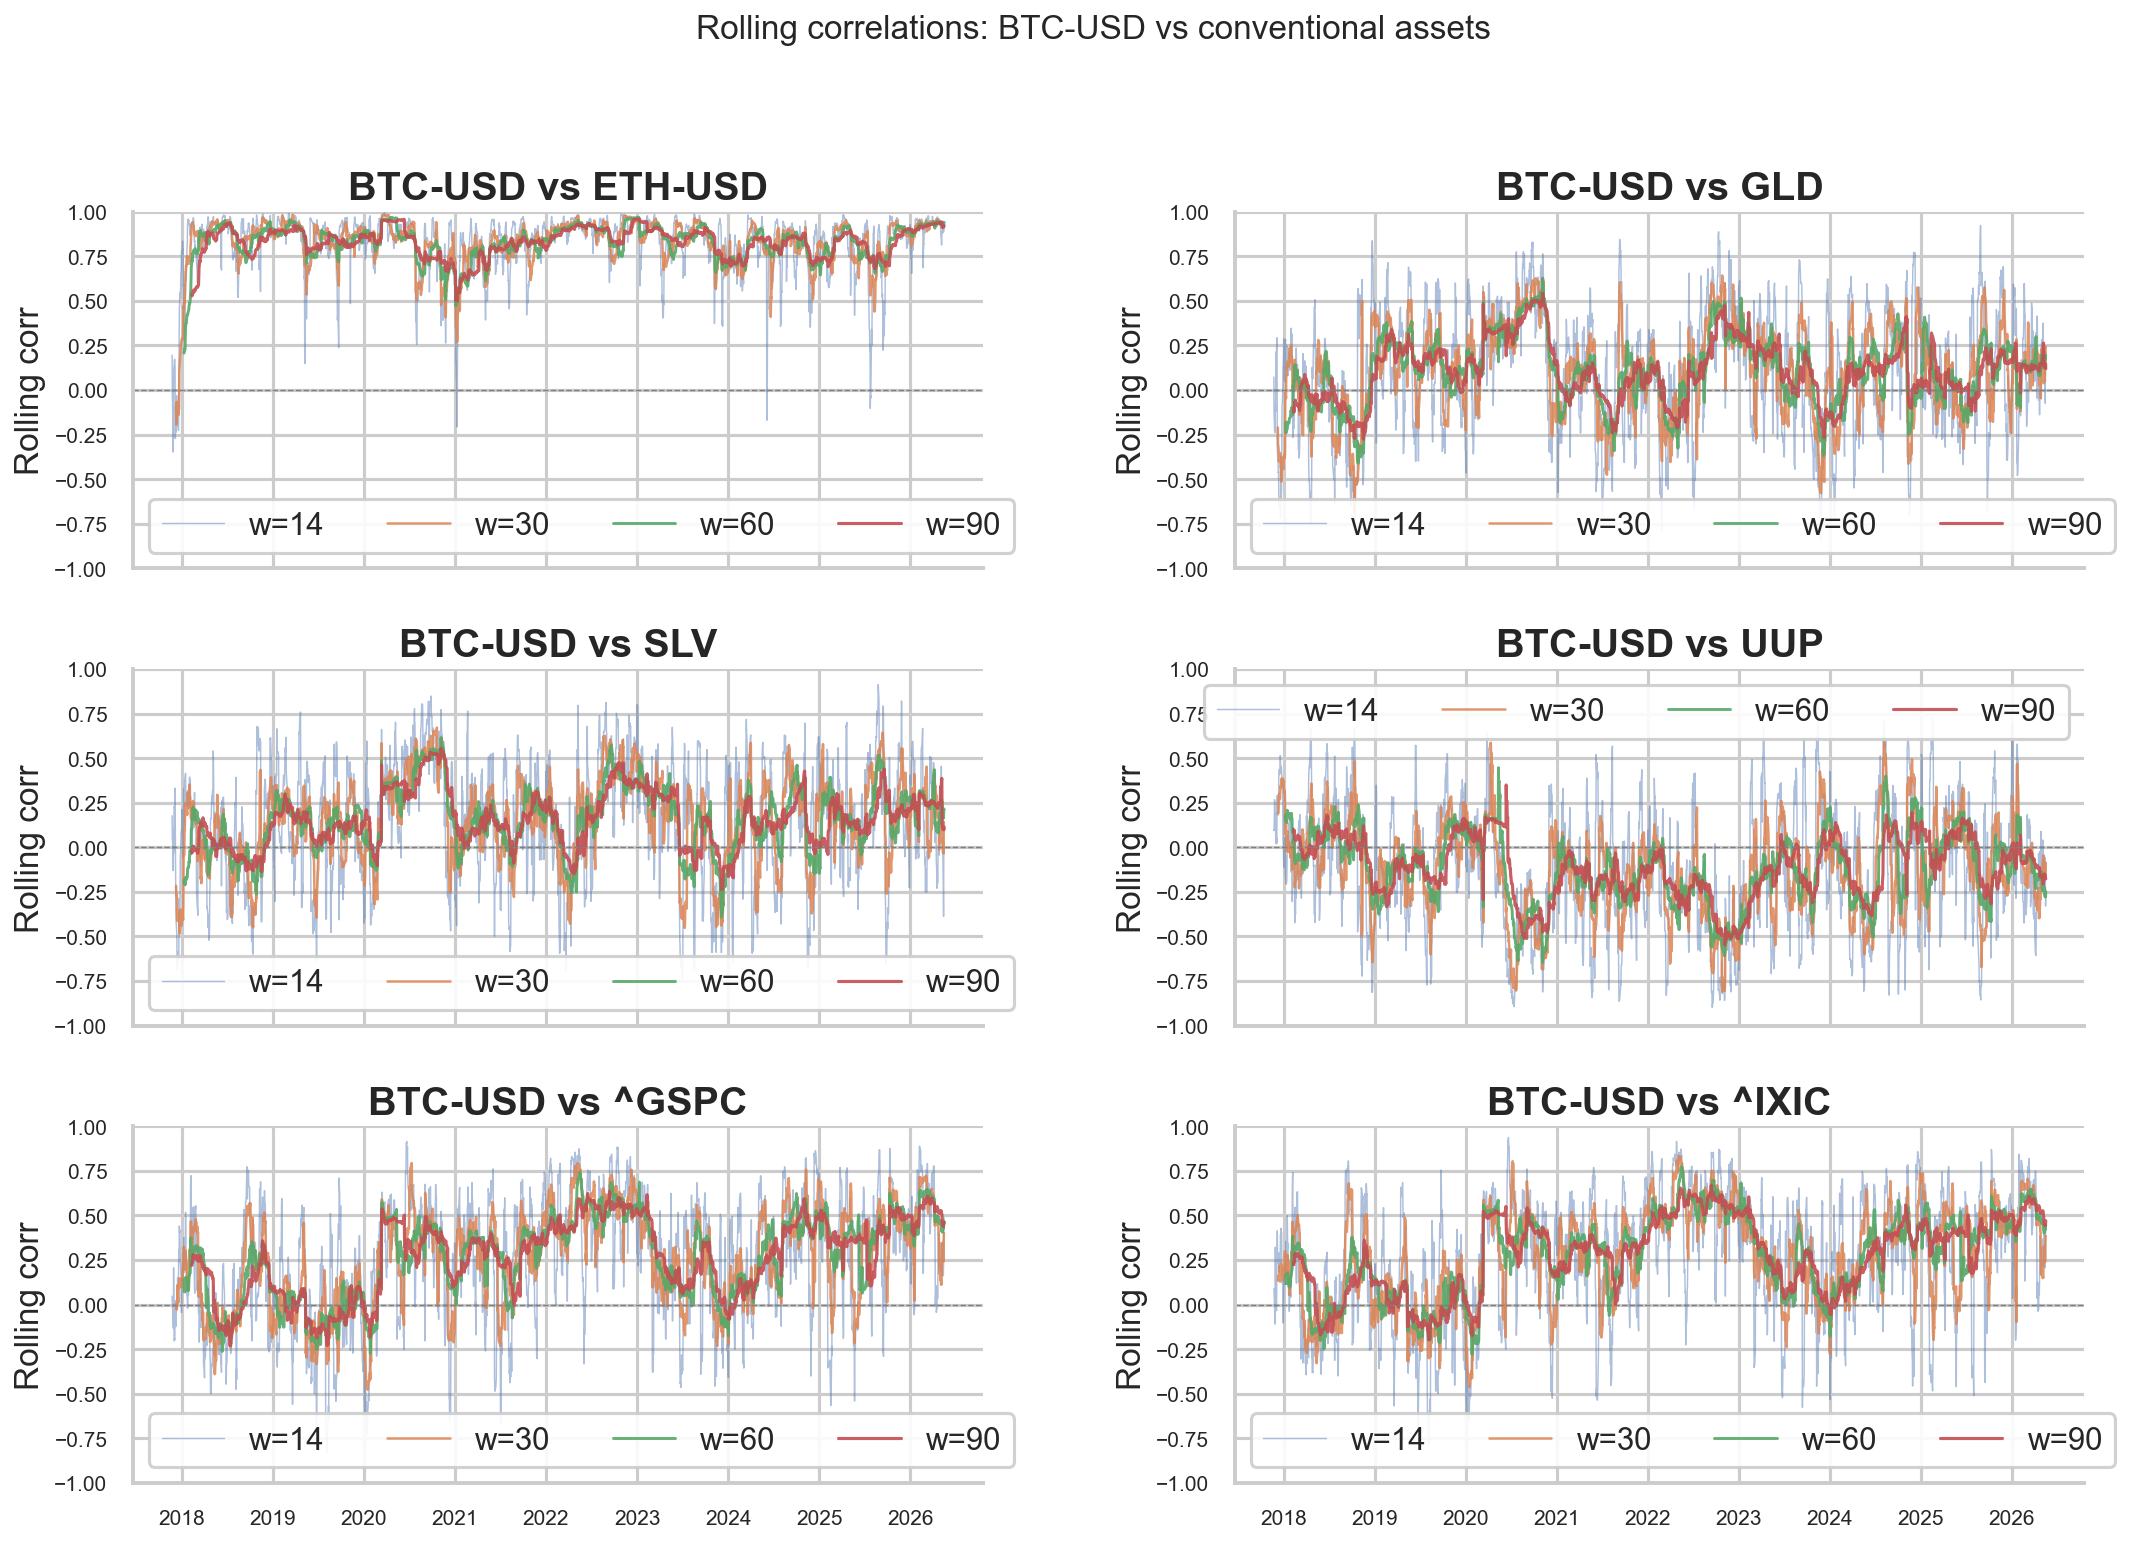
\includegraphics[width=0.95\textwidth, height=0.72\textheight, keepaspectratio]{../outputs/figures/eda_rolling_corr_all.png}
    \caption{Rolling dependency between Bitcoin and each of the five conventional assets plus Ethereum (six pairs in total) across all four window lengths (14, 30, 60, 90 days). The Fisher-transformed series exhibits the strong time-variation and persistence that motivate the forecasting framework.}
    \label{fig:rolling_corr_all}
\end{figure}

\subsection{Feature engineering}

The features are built around quantities a financial reader can interpret: a compact set of variables that could plausibly move future dependency, kept small enough to stay legible.

The features fall into several groups:

\begin{table}[H]
    \centering
    \caption{Main groups of predictors used in the dependency-forecasting layer.}
    \label{tab:feature_groups}
    \begin{tabular}{l p{0.55\textwidth}}
        \toprule
        Group & Description \\
        \midrule
        Dependency lags & Recent values of the rolling dependency target \\
        Dependency momentum \& regime & Trend (5- and 20-day change) and trailing z-score of the target \\
        Return lags & Lagged returns of Bitcoin and the paired asset \\
        Rolling means & Local average return over short windows \\
        Rolling volatility & Local standard deviation of returns \\
        Spread features & Absolute and signed gaps between crypto and asset behaviour \\
        Correlation regime gap & Short-window minus long-window correlation \\
        \bottomrule
    \end{tabular}
\end{table}

The dependency lags carry most of the predictive weight, because the target is persistent by construction. Dependency momentum (\texttt{dep\_mom}) and the trailing z-score (\texttt{dep\_zscore}) summarise the recent trend and the standardised level of the correlation. Return lags allow the models to respond to recent price direction, while the rolling-mean, volatility, and dispersion features describe the local risk regime. The regime gap (\texttt{corr\_diff}) measures how far short-term dependency has moved from its longer-term baseline, which can act as an early indicator of a regime shift. Listing~\ref{lst:features} shows how the feature matrix is assembled.

\begin{lstlisting}[language=Python, caption={Core feature engineering routine (\texttt{pipeline.py}; abbreviated --- the full routine additionally builds rolling-mean, dispersion, volatility-ratio, and lagged squared-return features).}, label=lst:features]
# Dependency lags (extended: up to quarterly)
for lag in [1, 2, 5, 10, 20, 60]:
    features[f"dep_lag{lag}"] = y_current.shift(lag)

# Dependency momentum (trend of the correlation series)
features["dep_mom_5"]  = y_current.diff(5)
features["dep_mom_20"] = y_current.diff(20)

# Dependency regime: z-score vs trailing 252-day history
features["dep_zscore"] = (y_current - dep_roll_mean) / (dep_roll_std + 1e-8)

# Volatility of both assets, at the pair window and at 60 days
features["vol_base"]     = returns[base].rolling(window).std()
features["vol_other"]    = returns[other].rolling(window).std()
features["vol_base_60"]  = returns[base].rolling(60).std()
features["vol_other_60"] = returns[other].rolling(60).std()

# Return lags for both assets
for lag in [1, 2, 5, 10, 20]:
    features[f"r_base_lag{lag}"]  = returns[base].shift(lag)
    features[f"r_other_lag{lag}"] = returns[other].shift(lag)

# Correlation regime gap: short-window minus long-window correlation
corr_short = rolling_corr(returns[base], returns[other], max(5, window // 4))
corr_long  = rolling_corr(returns[base], returns[other], window)
features["corr_diff"] = corr_short - corr_long
\end{lstlisting}

The signal layer takes the best available dependency forecast for the pair and combines it with a handful of crypto-derived predictors into a smaller, classification-oriented feature set. In effect, the second layer sees both the current state of the crypto market and where the dependency process is heading.

\subsection{Forecasting models}

\subsubsection{Baseline and autoregressive models}

Three persistence-based models anchor the set. The naive last-value baseline just carries the last observed value forward, with no fitting at all. AR(1) fits a single autoregressive lag by OLS. HAR (Heterogeneous AutoRegressive, after \textcite{corsi2009har}) adds two more horizons: the latest value, its five-day average (weekly), and its twenty-two-day average (monthly), fitted as a restricted OLS on the expanding window at each refit. These baselines are not a formality: because the target is persistent by construction, any more complex model must demonstrate a clear improvement over them to justify its use.

\subsubsection{Regularised linear models}

The linear block is Ridge and ElasticNet, each fitted after standardisation (regularisation is meaningless if the features sit on different scales). Both are specified in the notation of Eq.~(8): $\lambda$ is the penalty strength and $\alpha$ the $\ell_1/\ell_2$ mixing ratio, which scikit-learn's interface calls \texttt{alpha} and \texttt{l1\_ratio} respectively. Ridge ($\ell_2$, $\lambda = 0.5$) should do well when many predictors each carry a little signal. ElasticNet ($\lambda = 0.005$, $\alpha = 0.5$) is more aggressive and can zero out redundant lags outright.

\subsubsection{Tree ensembles and adaptive ensemble}

The non-linear block is Random Forest, \texttt{HistGradientBoostingRegressor} (a LightGBM-style histogram method, roughly ten times faster than the old gradient-boosting code), and XGBoost, which runs on the GPU when it can and quietly falls back to CPU when it cannot. On top of these sits an \texttt{Ensemble}: at each step it forms an inverse-RMSE weighted average of all the non-naive models, with the weights recomputed from the last 60 out-of-sample errors (during the first 60 steps, from whatever errors have accumulated so far).

The complete model set, ten specifications in total, is initialised as follows:

\begin{lstlisting}[language=Python, caption={Model definitions used in the walk-forward experiment (\texttt{pipeline.py}; simplified --- \texttt{Naive\_Last} and \texttt{HAR} are \texttt{None} here and are produced directly inside the walk-forward loop rather than through \texttt{.fit}).}, label=lst:models]
model_specs = {
    "Naive_Last": None,         # persistence baseline (no fit required)
    "AR(1)":        LinearRegression(),
    "HAR":        None,         # heterogeneous AR -- fitted via OLS on 3 lags
                                # (dep_lag1, avg5, avg22); see walk-forward loop
    "Ridge":      make_pipeline(StandardScaler(), Ridge(alpha=0.5)),
    "ElasticNet": make_pipeline(
                      StandardScaler(),
                      ElasticNet(alpha=0.005, l1_ratio=0.5, max_iter=5000)
                  ),
    "RF":  RandomForestRegressor(
               n_estimators=200, max_depth=10,
               min_samples_leaf=5, n_jobs=-1
           ),
    "GBM": HistGradientBoostingRegressor(     # LightGBM-style histogram algorithm
               max_iter=300, max_depth=4,
               learning_rate=0.02, min_samples_leaf=5,
               l2_regularization=0.1
           ),
    "XGB_GPU": xgb.XGBRegressor(
               device="cuda", n_estimators=500,
               max_depth=6, learning_rate=0.02,
               subsample=0.8, colsample_bytree=0.8
           ),
}
# "Ensemble": adaptive inverse-RMSE weighted average of the ML models
#             (excludes Naive_Last and the DCC-GARCH benchmark).
# Weights are recomputed at each step from the last 60 out-of-sample errors.
\end{lstlisting}

\subsubsection{DCC-GARCH benchmark}

The DCC-GARCH benchmark is implemented in a separate module and is leakage-safe by construction. Fitting DCC once on the full sample and then reading off ``out-of-sample'' predictions would use future information, so the benchmark is instead re-estimated on the training window alone and rolled forward from there. This is computationally slower, but it places the benchmark on the same out-of-sample footing as the machine-learning models.

\subsection{Investor signal layer}

The signal layer reformulates the problem as early-warning classification. The label is a \emph{stress day} for the conventional asset, not the direction of the next-day return. Day $t+1$ is labelled as stress if the asset's return falls below $-0.75\,\sigma_t$, where $\sigma_t$ is the trailing 20-day standard deviation of returns computed from information available at time $t$. This threshold produces a positive (stress) class of roughly 15--18\% of days, depending on the asset (15.2\% for the S\&P~500 up to 17.5\% for the dollar index), and its sensitivity is examined over the range $[0.5,\,2.0]\,\sigma$ in the robustness analysis. The threshold is chosen to capture moves that are worse than a typical down day without being limited to extreme tail events, which matches the downside-protection use case of the signal.

Three classifiers compete here: logistic regression, a random-forest classifier, and a gradient-boosted one. Each emits a probability, which is compared against a threshold to flag the next day as elevated-risk or not. The output is therefore a probability-guided warning, not an opaque buy/sell command.

\subsection{Walk-forward estimation framework}

Every experiment uses the same expanding-window walk-forward. Start with the first $T_0$ observations; at each origin $t \geq T_0$, fit on everything up to $t$ and predict $t+1$; continue to the end of the sample. Refitting happens periodically instead of at every step, which cuts the compute cost without ever breaking causal order.

\begin{lstlisting}[language=Python, caption={Expanding-window walk-forward loop (\texttt{pipeline.py}).}, label=lst:walkforward]
for t in range(min_train, n_obs):
    train_idx = np.arange(0, t)

    # Refit all models on the expanding training window periodically
    if (t - last_refit) >= refit_every:
        last_refit = t
        for name, model in model_specs.items():
            if model is not None:
                model.fit(X_values[train_idx], y_values[train_idx])
                fitted[name] = model

    # One-step-ahead prediction — uses only information up to t
    for name in fitted:
        preds[name][t] = fitted[name].predict(X_values[[t]])[0]
\end{lstlisting}

This design has three benefits: it reproduces realistic forecasting conditions, it keeps the benchmark comparison fair, and it produces a complete time series of out-of-sample errors. The last point is important, since those errors feed not only the average metrics but also the rolling diagnostics and the Diebold--Mariano tests.

\subsection{Evaluation metrics}

The forecasting layer is evaluated with three metrics: mean absolute error (MAE), root mean squared error (RMSE), and the out-of-sample $R^2$. Rankings are based on RMSE, which penalises large errors more heavily and is well suited to a smooth, continuous target.

For the signal layer, four numbers matter: Balanced Accuracy, the F1 score on the downside class, the area under the ROC curve (AUC), and the exit rate. Balanced Accuracy is emphasised because stress days are rare and the classes are imbalanced. The F1 score on the downside class keeps the focus on detecting the adverse days. The exit rate (how often the signal would move the investor out of the market) links statistical quality to how the signal would actually be used.

\subsection{Model comparison methodology}

When models are close, average metrics can mislead. So the thesis runs the Diebold--Mariano test on the loss series of selected pairs. The headline comparison is the best non-benchmark machine-learning model against DCC-GARCH; the secondary one pits that same model against the naive persistence baseline.

The setup is transparent by design. The thesis does not bury the possibility that the best model overall is a simple baseline; instead it uses the DM framework to separate three different levels of claim:

\begin{enumerate}
    \item whether dependency is forecastable at all,
    \item whether machine learning improves upon a classical econometric benchmark,
    \item whether machine learning adds value beyond persistence.
\end{enumerate}

A caveat applies to the second and third comparisons. When the simpler model is nested inside the richer one (as the naive baseline and AR(1) are inside Ridge or the tree ensembles), the standard Diebold--Mariano statistic is not strictly valid, because its asymptotic normal distribution assumes non-nested forecasts. Tests built for nested models, such as Clark--West or Giacomini--White \cite{clark2007nested,giacomini2006tests}, would be more rigorous, and the small-sample HLN correction reported in Appendix~E mitigates over-rejection but not nesting. The comparisons against the persistence baselines should therefore be read as indicative; the headline Ridge-versus-DCC-GARCH comparison, which is non-nested, is unaffected. A separate consideration concerns the variance estimator. The DM statistics use a Newey--West HAC estimator with zero lags, which is standard at the one-step horizon but assumes loss differentials that are not autocorrelated. Because the rolling-correlation target is built from overlapping windows, the loss differentials are autocorrelated by construction, so the zero-lag variance can be understated and the statistic correspondingly inflated. Re-estimating the variance with a lag of the order of the rolling-window length would give a more conservative statistic; given the very large margins against DCC-GARCH ($\mathrm{DM}\approx 27$), the significance of the headline comparison is unlikely to be overturned, but the precise magnitudes should be interpreted with this in mind.

The thesis organises its empirical conclusions around exactly these three levels.

\subsection{Implementation and reproducibility}

The whole workflow is Python, organised as a modular codebase. A main pipeline ties the steps together (read the config, compute returns, build targets and features, fit models, write prediction files, save figures, export \LaTeX\ tables), while separate modules handle the DCC walk-forward benchmark, notebook support, and the signal layer. This organisation is what makes the thesis reproducible end to end.

Everything lands in a structured output tree: metrics, DM tests, and signal results as CSV; thesis-ready tables as \LaTeX; diagnostics as figures. The point is to keep manual post-processing to a minimum and let the analysis feed the writing directly.

\subsection{Methodological expectations}

Before the results, it is worth saying what success would even look like. It does not mean finding a model that predicts every conventional market from Bitcoin; no serious forecasting study should promise that. A fairer bar has three parts: the dependency target should show out-of-sample forecastability, the benchmark comparison should establish whether machine learning improves on DCC-GARCH, and the signal layer should produce stress warnings that beat chance and can be acted on. These thresholds are modest on purpose.

Three further principles guide how the results are read. First, no single metric is treated as the verdict: the regression layer always reports RMSE, MAE, and $R^2$ together, and the classification layer reports Balanced Accuracy, F1, AUC, and exit rate together. Second, performance gaps are judged significant by the Diebold--Mariano test, not by eyeballing averages. Third, the analysis refuses to cherry-pick a window after the fact; all four (14, 30, 60, 90 days) are reported side by side, so no finding can rest on a lucky choice of specification.

Behind all three is the same commitment to methodological transparency. In-sample performance can appear strong yet deteriorate substantially under proper out-of-sample testing, and financial machine learning is unusually exposed to this failure, since repeated evaluation on the same historical sample inflates apparent performance long before any single result looks suspicious \cite{lopezdeprado2018advances}. The walk-forward design, the leakage-safe benchmark, and the all-windows evaluation together guard against the kind of inflated claims to which this literature is prone.
